\chapter{Apresentação e Análise dos Resultados}
O objeto deste trabalho é um sistema que faz o gerenciamento e a escalação automática de militares. O presente capítulo busca apresentar as funcionalidades implementadas no sistema e os passos necessários para realizar o build da aplicação.

\section{Sistema}

O sistema foi desevolvido utilizando o método de containerização, ou seja cada serviço tem o seu container. Para se construir a aplicação é necessário clonar o repositório, disponível \url{https://github.com/daniboyBr/tcc-escala-permanencia-v2}, e seguir os passos descritos no arquivo README.md. Após seguir todos os passos o sistema pode ser acesso em \url{http://localhost:8080}. Para se testar a aplicação a base de dados foi populada com dados fictícios, podemdo o perfil de administrador ser acessado com o e-mail "admin@permanencia.com" e a senha "123456789".

\subsection{Acessando o sistema}

A página inicial do sistema exibe o formulário de login, apresentada na \ref{fig:login}, é por meio dele que todo militar terá acessso as funcionalidades, sendo que algumas delas só é acessível para o usuário administrador do sistema.

\begin{figure}[!htb]
    \centering
    \caption{Tela de Login}
    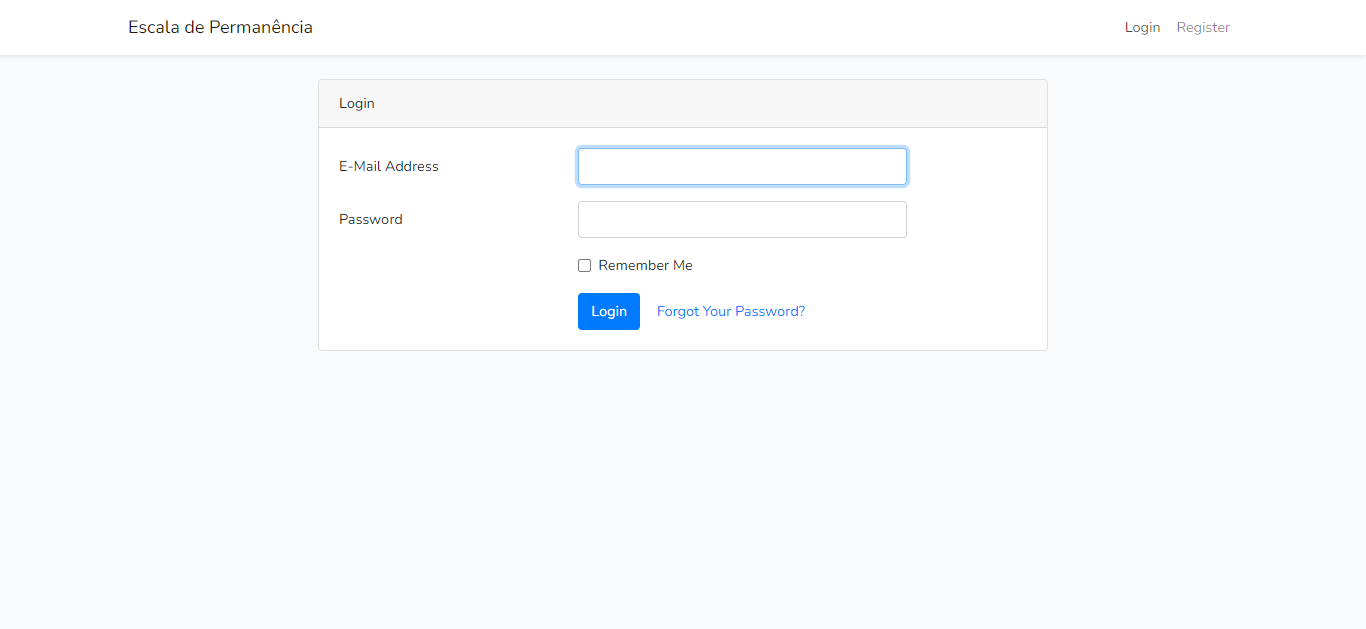
\includegraphics[width=0.8\textwidth]{images/1 - Pagina Inicial - Tela de Login.png}
    \label{fig:login}
\end{figure}

\section{Registrando-se no Sistema}

Na Figura \ref{fig:singnup} é mostrada a tela em que o militar deve realizar o seu cadastro, sendo que os campos e-mail e identidade devem ser únicos para cada militar.

\begin{figure}[!htb]
    \centering
    \caption{Tela de Cadastro de Militar}
    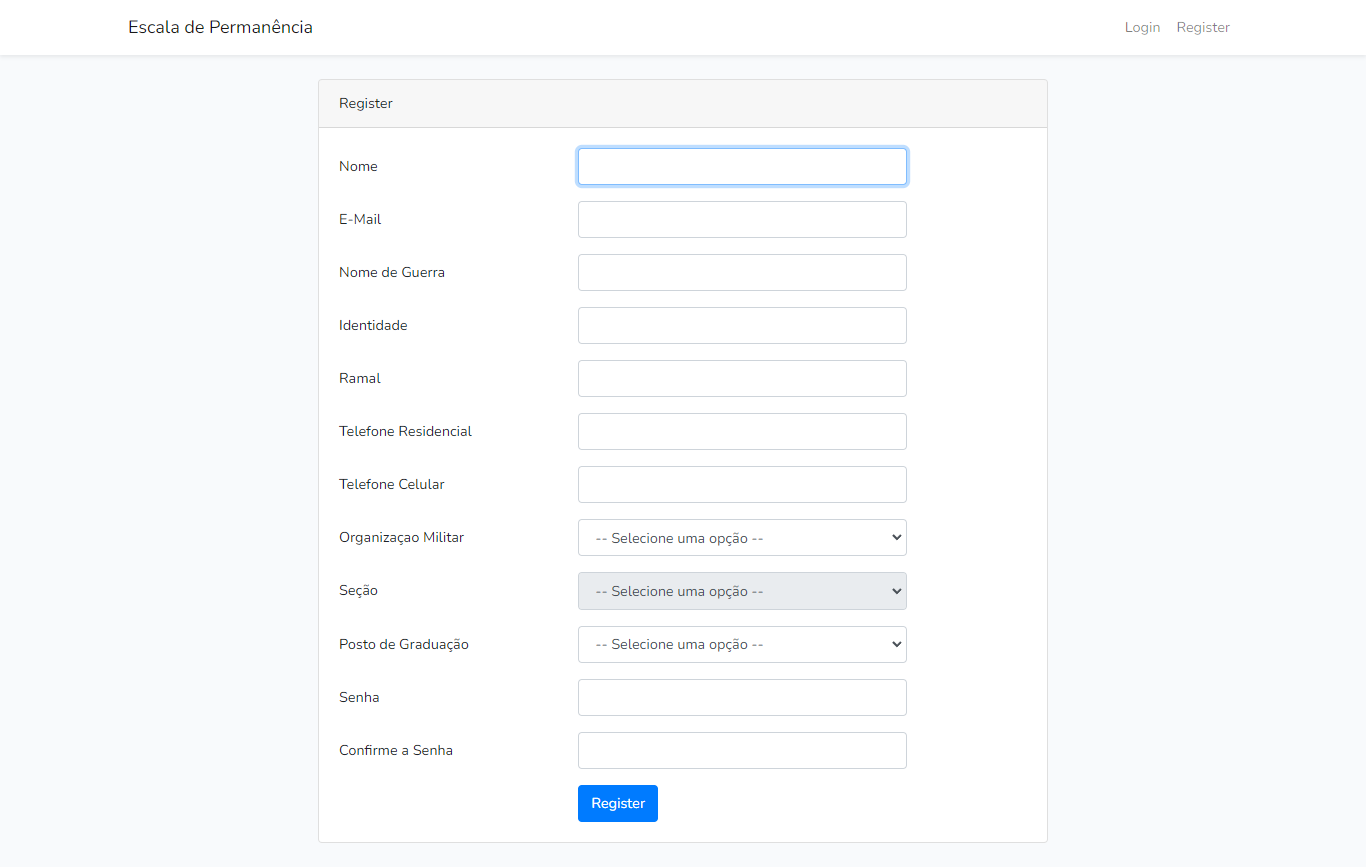
\includegraphics[width=0.8\textwidth]{images/2 - Tela de Cadastro.png}
    \label{fig:singnup}
\end{figure}

O militar, após ter efetuado cadastro, consegue ter acesso ao sistema, porém seu cadatro permanece inativo até que um usuário com perfil de administrador ativar seu cadastro, conforme apresentado na Figura \ref{fig:userinative}

\begin{figure}[!htb]
    \centering
    \caption{Tela de Militar Inativo}
    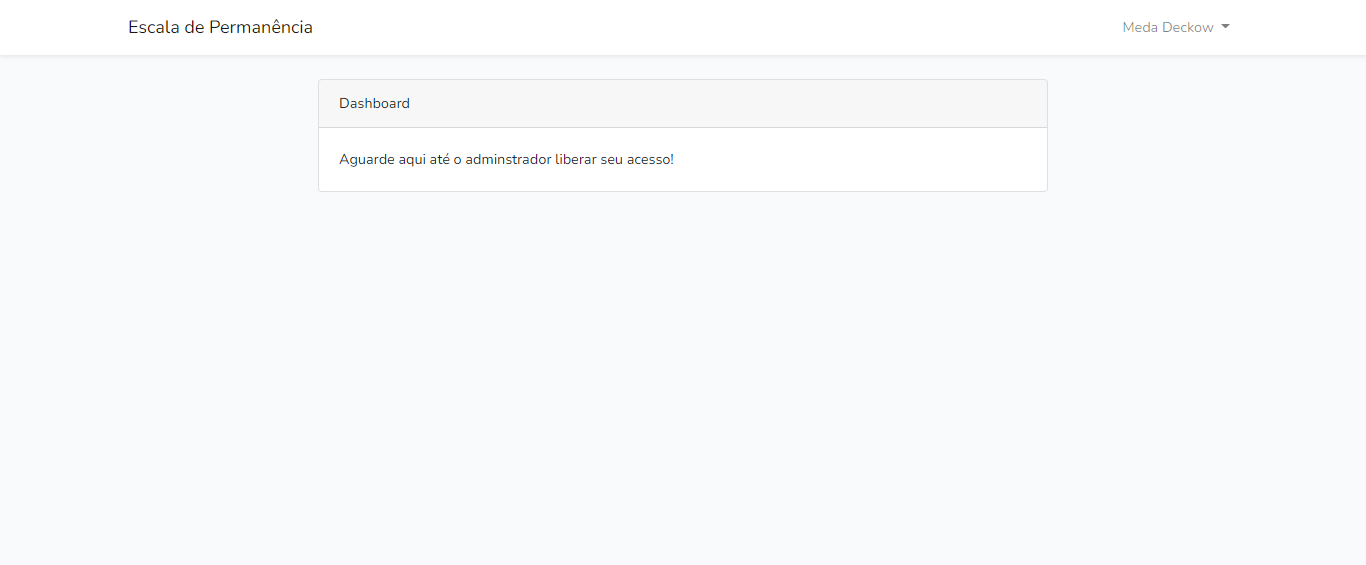
\includegraphics[width=0.8\textwidth]{images/3 - Tela de Militar Inativo.png}
    \label{fig:userinative}
\end{figure}

\subsection{Escala de Serviço}

Ao ter acesso ao sistema, com o cadastro ativo, o militar consegue visualizar a escala do dia corrente, tendo a possibilidade de pesquisar a escalação em datas futuras ou passadas por meio do filtro de data, conforme, apresentado na Figura \ref{fig:escalaservico}.

\begin{figure}[!htb]
    \centering
    \caption{Tela da Escala de Serviço}
    \includegraphics[width=0.8\textwidth]{images/4 - Tela de Visualizacao da Escala de Serviço.png}
    \label{fig:escalaservico}
\end{figure}

Na Figura \ref{fig:escalaservico}, é mostrado o botão livro, é através desse botão que o militar, no dia da sua escalação ao acessar o sistema, consegue relatar toda e qualquer ocorrência após o término do serviço, esse relato pode ser preechido no formulário apresentado na Figura \ref{fig:livroregistro}, uma vez registrado não se pode mais alterar a ocorrência informada.

\begin{figure}[!htb]
    \centering
    \caption{Tela Livro de Registro}
    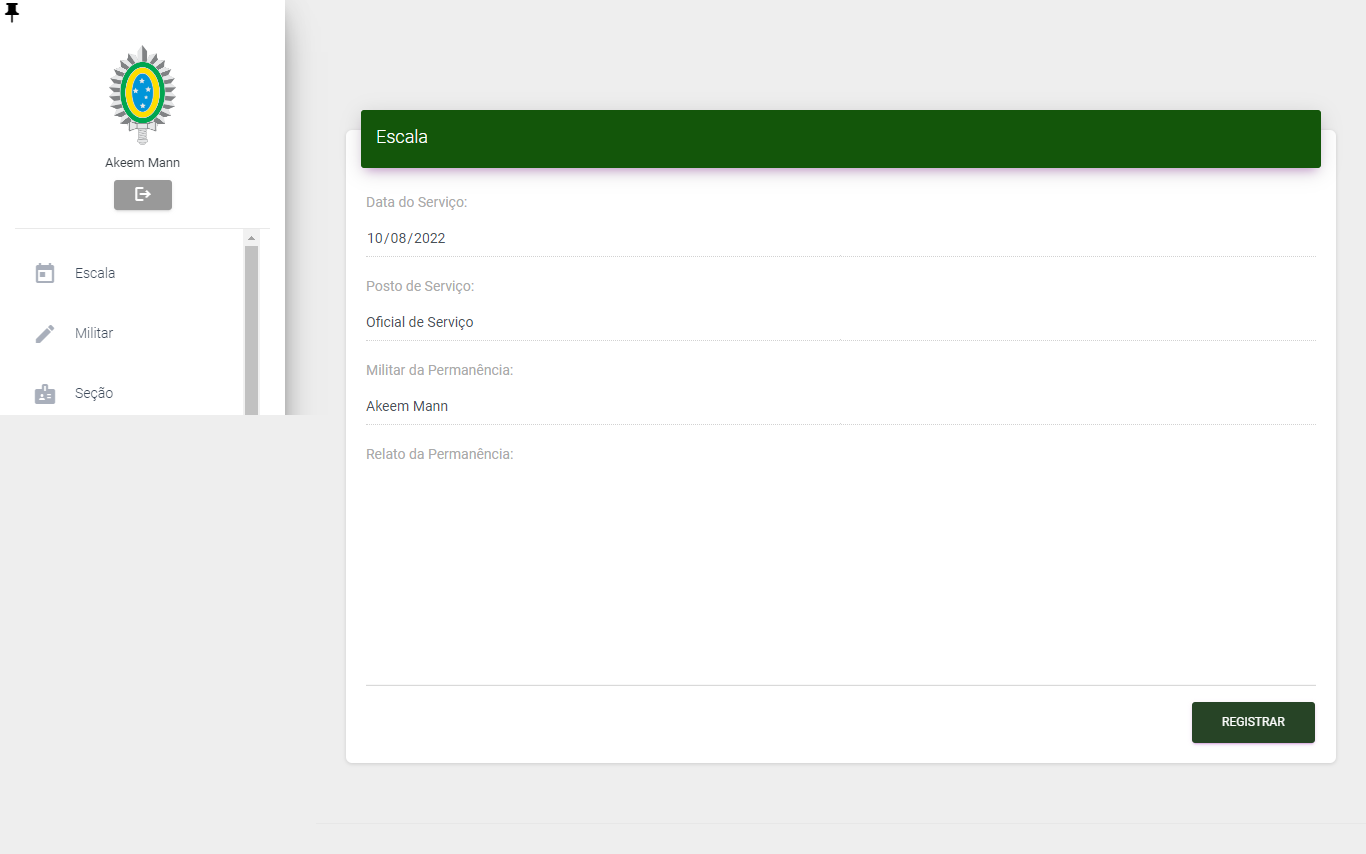
\includegraphics[width=0.8\textwidth]{images/5 - Tela Livo de Registro.png}
    \label{fig:livroregistro}
\end{figure}


\subsection{Gerar Escala}

A geração da escala acontece por debaixo dos panos. O Laravel disponibiliza uma classe chamada Command, a qual é necessário extender para criar um comando personalizado. Ao extender essa classe, foi implementadao o método handle, responsável por conter toda lógica para escalar os militares,  conforme apresentado no Algorítimo \ref{lst:algofirst}.

\begin{lstlisting}[frame=single, caption={Classe responsável por gerar escala}, label={lst:algofirst}]
class DailyScale extends Command
{
    protected $signature = 'scale:daily';
    /**  ommited code  */
    public function handle()
    {
        /**  logic to generate scale  */
    }
}
\end{lstlisting}

Ao se criar um comando personalizado no laravel, o mesmo ainda não é disparado de imediato, foi necessário configurá-lo na classe Kernel que extende de ConsoleKernel, para isso obrigatoriamente devemos informar um comando e a frequência na função shcedule, conforme mostrado no Algorítmo \ref{lst:algosecond}. A escalação automática foi configurada para rodar todo dia a meia noite.

\begin{lstlisting}[frame=single, caption={Configuração da geração da escala}, label={lst:algosecond}]
class Kernel extends ConsoleKernel
{
    protected $commands = [
        DailyScale::class
    ];
    protected function schedule(Schedule $schedule)
    {
        $schedule->command('scale:daily')->daily();
    }
    /**  ommited code  */
}
\end{lstlisting}
